

%\documentclass[12pt,a4paper]{article}
\documentclass[tikz]{standalone}

\usepackage[english]{babel}
\usepackage[utf8]{inputenc}
\usepackage{amsfonts,amssymb,amsbsy}
\usepackage{xcolor}

\usepackage{tikz}
\usetikzlibrary{arrows.meta, positioning, quotes, calc, intersections, decorations.pathreplacing}

\begin{document}

	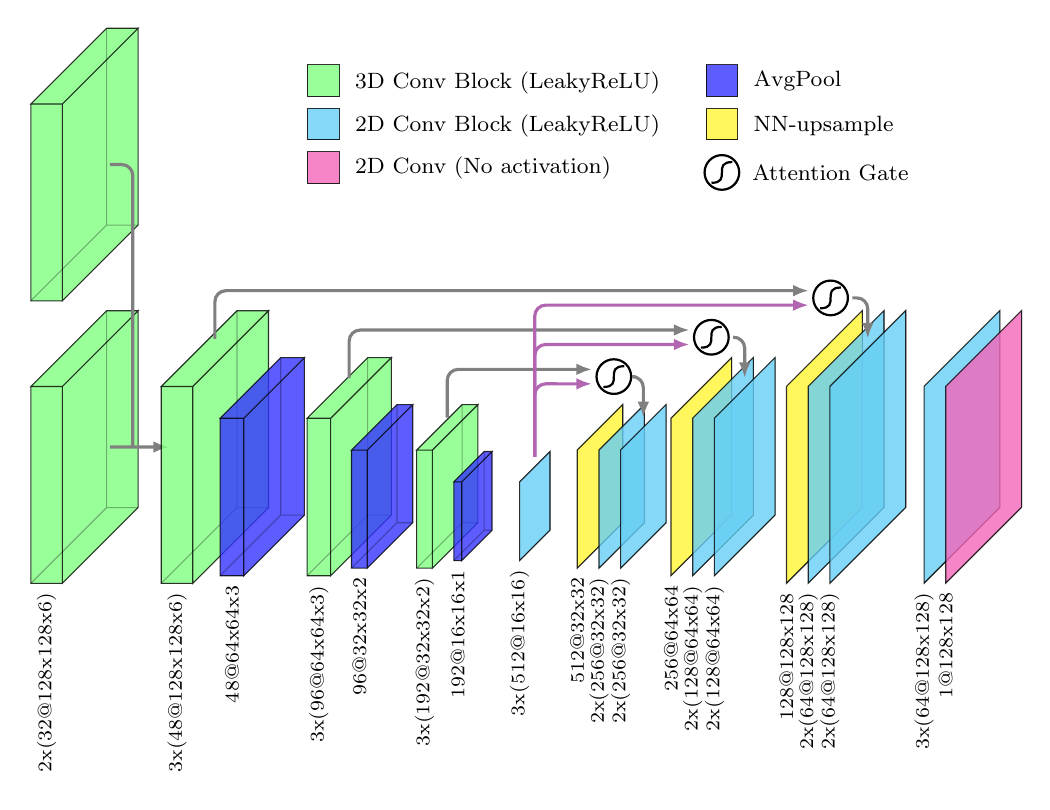
\begin{tikzpicture}[scale=0.92]
	
	\tikzset{
		cuboid/.pic={
			\tikzset{%
				every edge quotes/.append style={midway, auto},
				/cuboid/.cd,
				#1
			}
			\draw [every edge/.append style={pic actions, densely dashed, opacity=.5}, pic actions]
			(0,0,0) coordinate (sl) ++(0,\cubescale*\cubey,\cubescale*\cubez/2) coordinate (o)
			-- ++(-\cubescale*\cubex,0,0) coordinate (a) -- ++(0,-\cubescale*\cubey,0) coordinate (b) -- node[midway] (bm) {} ++(\cubescale*\cubex,0,0) coordinate (c) -- node[midway] (fm) {} cycle
			(o) -- node[midway] (su1) {} ++(0,0,-\cubescale*\cubez) coordinate (d) -- ++(0,-\cubescale*\cubey,0) coordinate (e) -- (c) -- cycle
			(o) -- (a) -- node[midway] (su2) {} ++(0,0,-\cubescale*\cubez) coordinate (f) -- (d) -- cycle
			($(su1)!0.5!(sl)$) node (sc) {}
			($(su1)!0.5!(su2)$) node (uc) {};
			\path (uc) ++($(b)-(a)$) coordinate(bc);
			\draw [opacity=0.3] (f) -- ++(0,-\cubescale*\cubey,0) coordinate(g) (g) -- (e) (g) -- (b);
		},
		pics/attsymbol/.style args={#1, #2}{
			code={
				\def\r{0.6*#1}
				\draw[black, line width=#2] circle (#1) coordinate (c);
				\draw[black, line width=#2] (-\r, -\r) .. controls (\r, -\r, 0) and (-\r, \r) .. (\r, \r);
			}
		},
		conv3d/.pic={\pic [fill=green!50!white, opacity=0.8] {cuboid={#1}};},
		conv2d/.pic={\pic [fill=magenta!60!white, opacity=0.8] {cuboid={#1}};},
		conv2dlr/.pic={\pic [fill=cyan!60!white, opacity=0.8] {cuboid={#1}};},
		conv2dr/.pic={\pic [fill=blue!50!white, opacity=0.8] {cuboid={#1}};},
		upsample/.pic={\pic [fill=yellow!80!white, opacity=0.8] {cuboid={#1}};},
		maxpool/.pic={\pic [fill=blue!80!white, opacity=0.8] {cuboid={#1}};},
		avgpool/.pic={\pic [fill=teal!80!white, opacity=0.8] {cuboid={#1}};},
		myline/.style={draw=black!50!white, line width=0.4mm, rounded corners},
		myarrow/.style={myline, -{Latex[width=0.15cm, length=0.2cm]}},
		myarrow2/.style={myline, draw=violet!60!white, -{Latex[width=0.15cm, length=0.2cm]}},
		layerparam/.style={rotate=90, anchor=east, font=\scriptsize},
		/cuboid/.search also={/tikz},
		/cuboid/.cd,
		width/.store in=\cubex,
		height/.store in=\cubey,
		depth/.store in=\cubez,
		units/.store in=\cubeunits,
		scale/.store in=\cubescale,
		width=1,
		height=1,
		depth=1,
		units=cm,
		scale=1
	}
	
	% Input branches
	\path (0,0,0) coordinate (model) pic {conv3d={width=0.4, height=2.5, depth=2.5}} (sc) node (c1) {} (sl)
	++(0,-3.9,0) pic {conv3d={width=0.4, height=2.5, depth=2.5}} (sc) node (c2) {}
	(bm) node[layerparam] {2x(32@128x128x6)} (sl);
	
	% Input branch arrows
	\draw[myarrow] (c2) -- ++(0.95, 0);
	\draw[myline] (c1) -- ++(0.45,0) -- ++($(c2)-(c1)$);
	
	% Encoder
	\path ($(sl)+(1.8,0,0)$) pic {conv3d={width=0.4, height=2.5, depth=2.5}} (uc) node (c3) {} (bc) node (c3b) {} (sl)
	(bm) node[layerparam] {3x(48@128x128x6)} (sl)
	++(0.6,0,0) pic {maxpool={width=0.3, height=2.0, depth=2.0}}
	(bm) node[layerparam] {48@64x64x3} (sl)
	%
	++(1.2,0,0) pic {conv3d={width=0.3, height=2.0, depth=2.0}} (uc) node (c4) {} (bc) node (c4b) {} (sl)
	(bm) node[layerparam] {3x(96@64x64x3)} (sl)
	++(0.4,0,0) pic {maxpool={width=0.2, height=1.5, depth=1.5}}
	(bm) node[layerparam] {96@32x32x2} (sl)
	% 
	++(0.9,0,0) pic {conv3d={width=0.2, height=1.5, depth=1.5}} (uc) node (c5) {} (bc) node (c5b) {} (sl)
	(bm) node[layerparam] {3x(192@32x32x2)} (sl)
	++(0.3,0,0) pic {maxpool={width=0.1, height=1.0, depth=1.0}}
	(bm) node[layerparam] {192@16x16x1} (sl)
	
	% Middle
	++(0.8,0,0) pic {conv2dlr={width=0, height=1.0, depth=1.0}} (uc) node (m1) {} (sl) node (m1b) {}
	(bm) node[layerparam] {3x(512@16x16)} (sl)
	
	% Decoder
	++(0.9,0,0) pic {upsample={width=0, height=1.5, depth=1.5}}
	(bm) node[layerparam] {512@32x32} (sl)
	++(0.3,0,0) pic {conv2dlr={width=0, height=1.5, depth=1.5}}
	(bm) node[layerparam] {2x(256@32x32)} (sl)
	++(0.3,0,0) pic {conv2dlr={width=0, height=1.5, depth=1.5}} (uc) node (c6) {} (sl)
	(bm) node[layerparam] {2x(256@32x32)} (sl)
	%
	++(0.8,0,0) pic {upsample={width=0, height=2.0, depth=2.0}}
	(bm) node[layerparam] {256@64x64} (sl)
	++(0.3,0,0) pic {conv2dlr={width=0, height=2.0, depth=2.0}} 
	(bm) node[layerparam] {2x(128@64x64)} (sl)
	++(0.3,0,0) pic {conv2dlr={width=0, height=2.0, depth=2.0}} (uc) node (c7) {} (sl)
	(bm) node[layerparam] {2x(128@64x64)} (sl)
	%
	++(1.1,0,0) pic {upsample={width=0, height=2.5, depth=2.5}}
	(bm) node[layerparam] {128@128x128} (sl)
	++(0.3,0,0) pic {conv2dlr={width=0, height=2.5, depth=2.5}}
	(bm) node[layerparam] {2x(64@128x128)} (sl)
	++(0.3,0,0) pic {conv2dlr={width=0, height=2.5, depth=2.5}} (uc) node (c8) {} (sc) node (c9) {}
	(bm) node[layerparam] {2x(64@128x128)} (sl);
	
	% Output branches
	\path ($(sl)+(1.3,0,0)$) pic {conv2dlr={width=0, height=2.5, depth=2.5}}
	(bm) node[layerparam] {3x(64@128x128)} (sl)
	++(0.3,0,0) pic {conv2d={width=0, height=2.5, depth=2.5}}
	(bm) node[layerparam] {1@128x128} (sl);
	
	% Skip-connections
	\def\dy{0.1}
	\draw[myarrow] (c5) -- ++(0.0,0.8,0) coordinate (s1) -- ++(2, 0) coordinate (a1);
	\path ($(a1)+(0.3, -0.1)$) pic {attsymbol={0.22, 0.8}} ++(0.3, 0)  coordinate (a2);
	\draw[myarrow2] (m1) -- ($(s1)+(m1b)-(c5b)-(0.0,2*\dy)$) -- ($(a1) - (0, 2*\dy)$);
	\draw[myarrow] (a2) -- ++($(c6)-(a2)+(s1)-(c5)-(0,\dy)$) -- (c6);
	%
	\draw[myarrow] (c4) -- ++(0.0,0.8,0) coordinate (s1) -- ++(4.7, 0) coordinate (a1);
	\path ($(a1)+(0.3, -0.1)$) pic {attsymbol={0.22, 0.8}} ++(0.3, 0)  coordinate (a2);
	\draw[myarrow2] (m1) -- ($(s1)+(m1b)-(c4b)-(0.0,2*\dy)$) -- ($(a1) - (0, 2*\dy)$);
	\draw[myarrow] (a2) -- ++($(c7)-(a2)+(s1)-(c4)-(0,\dy)$) -- (c7);
	%
	\draw[myarrow] (c3) -- ++(0.0,0.8,0) coordinate (s1) -- ++(8.2, 0) coordinate (a1);
	\path ($(a1)+(0.3, -0.1)$) pic {attsymbol={0.22, 0.8}} ++(0.3, 0)  coordinate (a2);
	\draw[myarrow2] (m1) -- ($(s1)+(m1b)-(c3b)-(0.0,2*\dy)$) -- ($(a1) - (0, 2*\dy)$);
	\draw[myarrow] (a2) -- ++($(c8)-(a2)+(s1)-(c3)-(0,\dy)$) -- (c8);
	
	% Legend
	\path (model) ++(3.3,2.3,0) coordinate (start)
	pic {conv3d={width=0.4, height=0.4, depth=0}} ($(fm)+(-0.05,-0.03)$) node [label=east:{\footnotesize 3D Conv Block (LeakyReLU)}] {} (sl)
	++(0,-0.6,0) pic {conv2dlr={width=0.4, height=0.4, depth=0}} ($(fm)+(-0.05,-0.03)$) node [label=east:{\footnotesize 2D Conv Block (LeakyReLU)}] {} (sl)
	++(0,-0.6,0) pic {conv2d={width=0.4, height=0.4, depth=0}} ($(fm)+(-0.05,-0.01)$) node [label=east:{\footnotesize 2D Conv (No activation)}] {} (bm)
	(start) ++(5.5,0,0) pic {maxpool={width=0.4, height=0.4, depth=0}} ($(fm)+(-0.05,-0.01)$) node [label=east:{\footnotesize AvgPool}] {} (sl)
	++(0,-0.6,0) pic {upsample={width=0.4, height=0.4, depth=0}} ($(fm)+(-0.05,-0.03)$) node [label=east:{\footnotesize NN-upsample}] {} (bm)
	++(0,-0.45,0) pic {attsymbol={0.22, 0.8}} ($(c)+(0.15, 0)$) node [label=east:{\footnotesize Attention Gate}] {};
	
	\end{tikzpicture}
	
	
\end{document}